\documentclass[../main.tex]{subfiles}
\graphicspath{
    {"../img/"}
    {"img/"}
}

\begin{document}
    \subsection{Ostatnio}
    Była rozmaitość $M$ z wymiarem $\dim M = n$, krzywa
    \[
        L : \left\{ [a,b]\ni t \to \varphi(t)\in \mathbb{R}^n \right\}
    ,\]
jednoforma $\omega \in \Lambda^1M$ i zastanawialiśmy się jak obliczyć
\[
\int_L\omega = \int_a^b\left<\varphi^\star \omega, \pm\frac{\partial }{\partial t}  \right>dt
.\]
Wyszło nam dla $\omega = ydx$,
 \[
\int_{C_1}\omega = 2,\quad \int_{C_2}\omega = -2
.\]
(rys 9)
\begin{figure}[h]
    \centering
    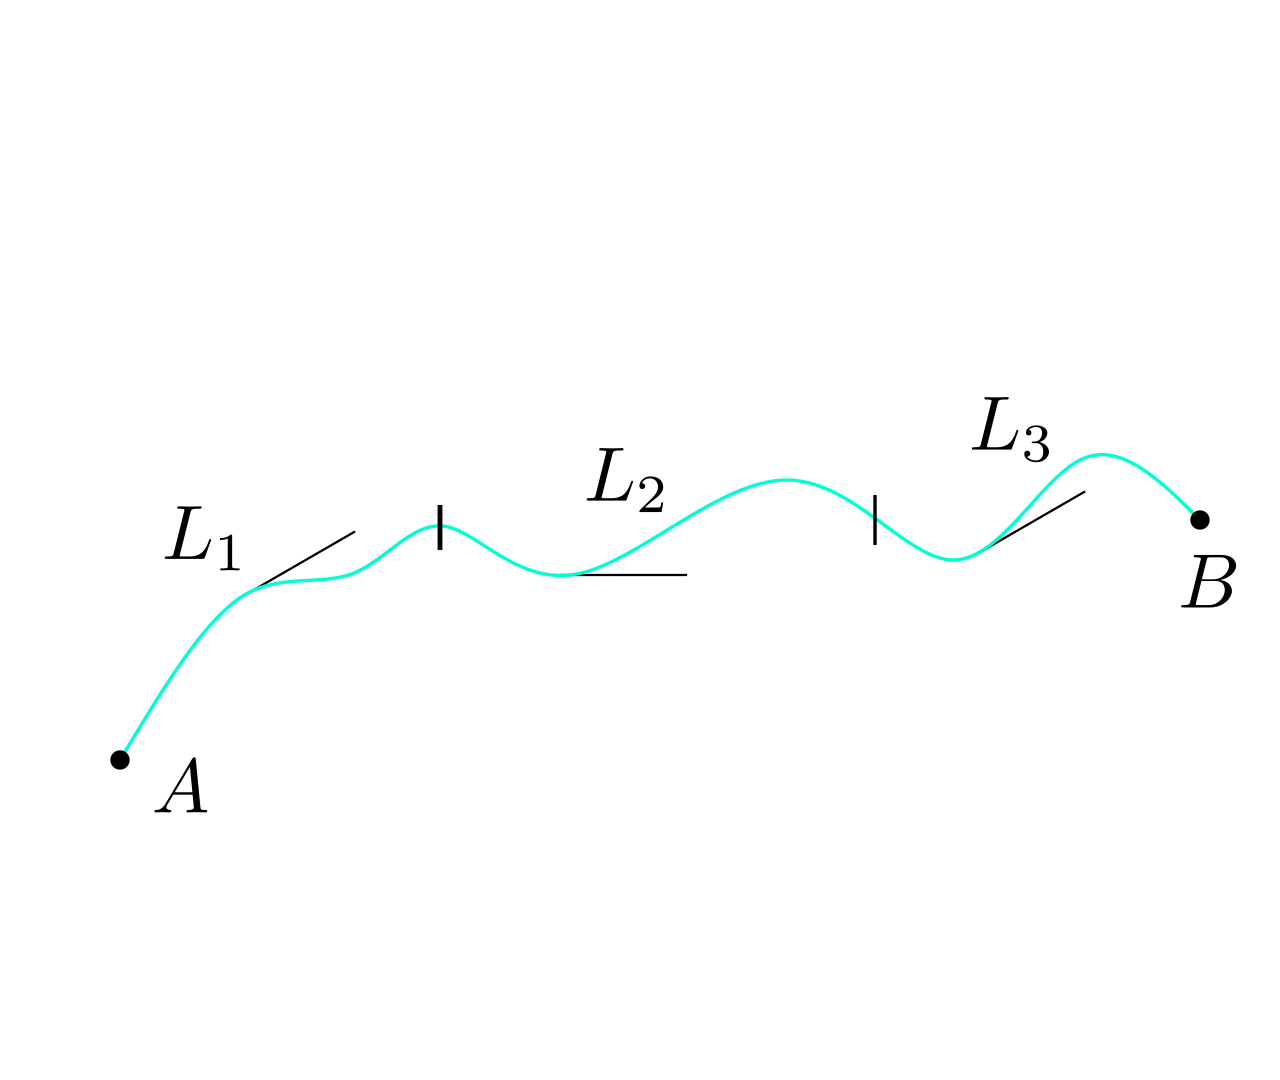
\includegraphics[width=0.4\textwidth]{fig2-1}
    \caption{W każdym momencie chcemy wiedzieć, w którą stronę chcemy iść. $L_1 + L_2 + L_3 = L$}
    \label{fig:fig2-1}
\end{figure}
\begin{przyklad}
    (rys 10)
    \begin{figure}[h]
        \centering
        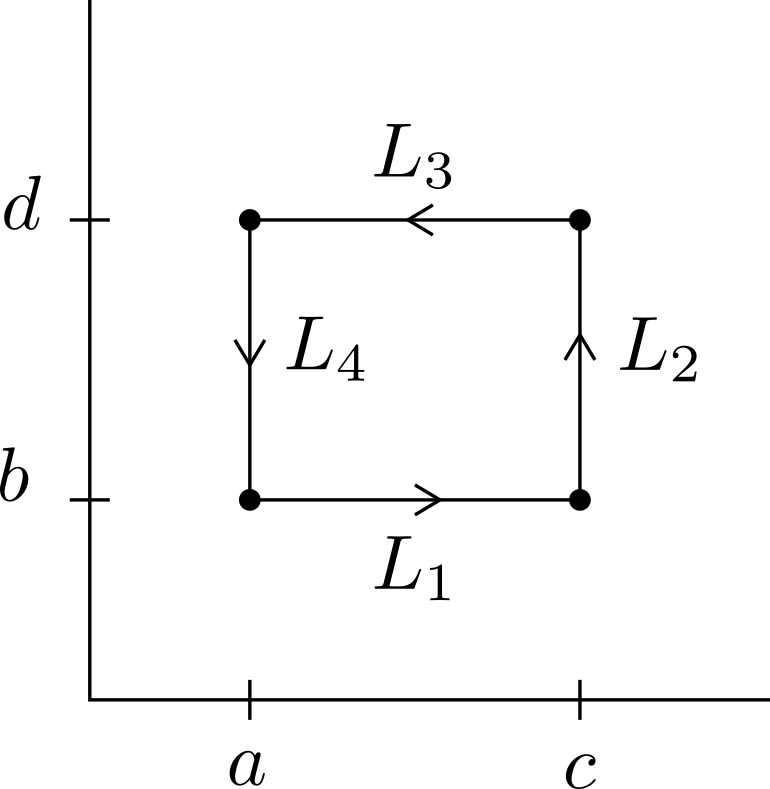
\includegraphics[width=0.3\textwidth]{fig2-2}
        \caption{$\dim M = 2$}
        \label{fig:fig2-2}
    \end{figure}
    \[
        \omega = A(x,y)dx + B(x,y)dy\in \Lambda^1M
    .\]
Trzeba te krzywe sparametryzować:
\[
    L_1 = \left\{ (x,b), a \le x \le c \right\}
.\]
\[
    L_2 = \left\{ (c,y), b \le y \le d \right\}
.\]
\[
    L_3 = \left\{ (x,d), a \le x \le c \right\}
.\]
\[
    L_4 = \left\{ (a,y), b \le y \le d \right\}
.\]
\begin{align*}
    \int_L\omega &= \int_{L_1}\omega + \int_{L_2}\omega + \int_{L_3}\omega + \int_{L_4}\omega =\\
    &= \int_a^c\left<\varphi_1^\star\omega, \frac{\partial }{\partial x}  \right>dx + \int_b^d\left<\varphi_2^\star \omega, \frac{\partial }{\partial y}  \right>dy + \int_a^c\left<\varphi^\star_3\omega, -\frac{\partial }{\partial x}  \right>dx + \int_b^d\left<\varphi_4^\star \omega, -\frac{\partial }{\partial y}  \right> =\\
    &= \int_a^c A(x,b)dx + \int_b^d B(c,y)dy + (-1)\cdot \int_a^cA(x,d)dx + (-1)\cdot \int_b^dB(a,y)dy
.\end{align*}
\end{przyklad}
(rys 11)\\
\begin{figure}[h]
    \centering
    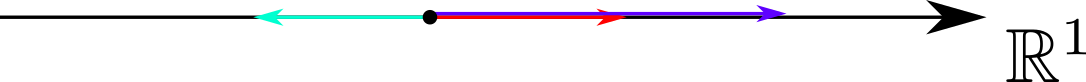
\includegraphics[width=0.5\textwidth]{fig2-3}
    \caption{Tramwaj nie ma za dużo możliwości, jedynie przód, tył i ewentualnie szybciej - na rolkach}
    \label{fig:fig2-3}
\end{figure}
dla $\dim M = \mathbb{R}^1$. Niech $\varphi : T_pM \to T_pM$, $\varphi(v) = a\cdot v$ ($\varphi$ - liniowe).\\
$a > 0$ - nie zmienia orientacji (kierunku)\\
$a < 0$ - zmienia kierunek wektora.

(rys 12)
\begin{figure}[h]
    \centering
    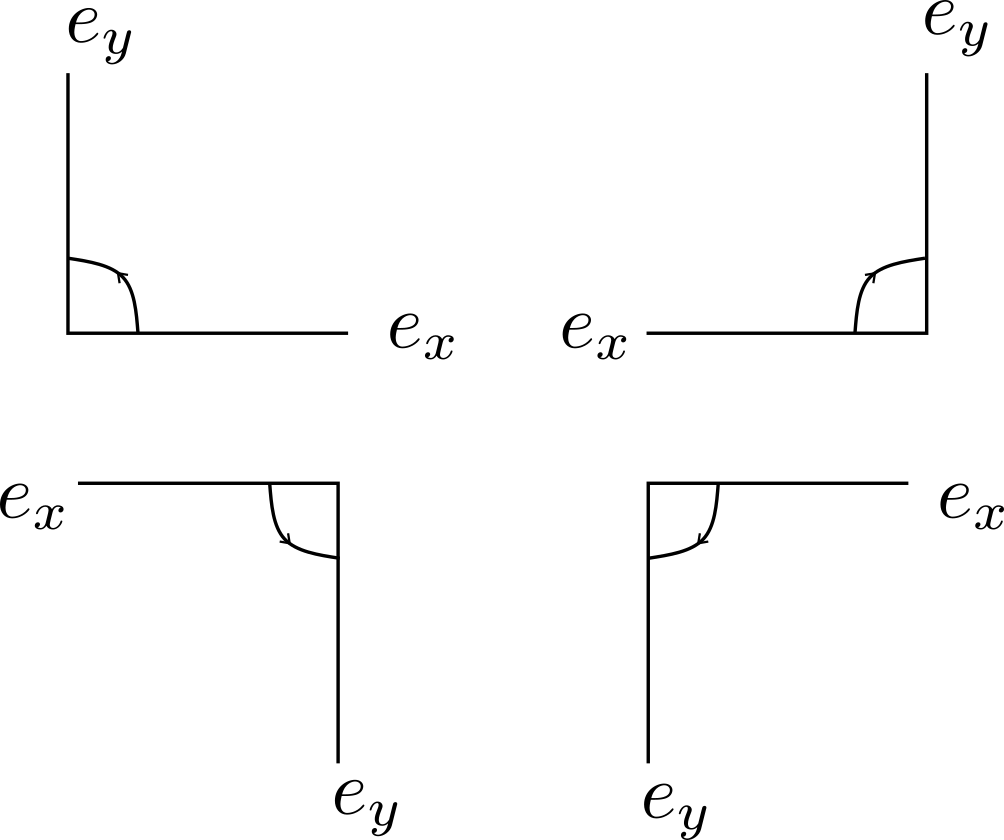
\includegraphics[width=0.4\textwidth]{fig2-4}
    \caption{Różne orientacje na $\mathbb{R}^2$, czy można to jakoś pogrupować?}
    \label{fig:fig2-4}
\end{figure}
\begin{definicja}
    Niech $B_1$, $B_2$ - bazy uporządkowane w $V$ - przestrzeń wektorowa. Mówimy, że $B_1$ i $B_2$ należą do tej samej klasy orientacji, jeżeli wyznacznik odwzorowania liniowego z $B_1$ do $B_2$ jest większy od zera.\\
    Wybór klasy orientacji nazywamy zorientowaniem $V$.
\end{definicja}
\begin{definicja}
    Orientacją standardową na $\mathbb{R}^n$ nazywamy wybór zgodny z bazą standardową, tzn.
    \[
        e_1 = \begin{bmatrix} 1\\0\\0\\ \vdots \end{bmatrix},\quad e_2 = \begin{bmatrix} 0\\1\\0\\ \vdots \end{bmatrix},\quad e_3 = \ldots
    .\]
\end{definicja}

\pagebreak
\begin{definicja}
    Niech $M$ - rozmaitość zorientowana, $\dim M = n$ i \\
    $S = \left\{ [a,b]\times[c,d]\ni (t_1,t_2) \to \varphi(t_1,t_2)\in M \right\}$ - powierzchnia sparametryzowana, $\Lambda^2M\ni\omega$ - dwuforma. Wówczas
    \[
        \int_S \omega \overset{\text{def}}{=} \int_a^b\int_c^d \left<\varphi^\star\omega, \underbrace{\pm \frac{\partial }{\partial t_1} , \pm \frac{\partial }{\partial t_2}}_\text{zgodne z orientacją}\right>dt_1dt_2
    .\]
\end{definicja}
\begin{przyklad}
    do 7:\\
    weźmy $\omega = A(x,y)dx + B(x,y)dy$ i obliczmy $\int\int_P d\omega$.
     \[
         d\omega = \frac{\partial A}{\partial y} dy\land dx + \frac{\partial B}{\partial x} dx\land dy = \left(\frac{\partial B}{\partial x} - \frac{\partial A}{\partial y} \right)dx\land dy
    ,\]
\[
    P = \left\{ (x,y)\in \mathbb{R}^2: \begin{matrix}a\le x\le b\\ c\le y \le d \end{matrix} \right\}
.\]
Wtedy mamy
\begin{align*}
    \int\int_P d\omega &= \int\int_{[a,b]\times[c,d]} \left<d\omega, \frac{\partial }{\partial x} , \frac{\partial }{\partial y}  \right> = \\
    &= \int_a^b dx \int_c^d dy\left(\frac{\partial B}{\partial x} - \frac{\partial A}{\partial y} \right) = \int_c^d dy\int_a^b \frac{\partial B(x,y)}{\partial x} dx - \int_a^bdx\int_c^ddy \frac{\partial A}{\partial y} = \\
    &= \int_c^d dy(B(b,y) - B(a,y)) - \left[ \int_a^bdx \left( A(x,d) - A(x,c) \right)  \right] = \\
    &= \int_a^bA(x,c)dx + \int_c^dB(b,y)dy - \int_a^cA(x,d)dx - \int_c^dB(a,y)dy =\\
    &= \int_{L_1}\omega + \int_{L_2}\omega + \int_{L_3}\omega + \int_{l_4}\omega
.\end{align*}
Czyli \[
\int\int_Pd\omega = \int_L \omega
,\]
to kiedyś będzie twierdzenie Stokesa
\end{przyklad}
\begin{przyklad}
    niech (sytuacja jak na rys 13) $S = S_1\cup S_2$, gdzie
    \[
        S_1 = \left\{ (x,y,z)\in \mathbb{R}^3, x^2 + y^2 + z^2 = 1, z\ge 0 \right\},\quad S_2 = \left\{ (x,y,z)\in \mathbb{R}^3, x^2+y^2 \le 1, z = 0 \right\}
    ,\]
$\alpha\in \Lambda^2M$.
\[
\int_S \alpha = \int_{S_1}\alpha + \int_{S_2}\alpha
.\]
    \begin{figure}[h]
        \centering
        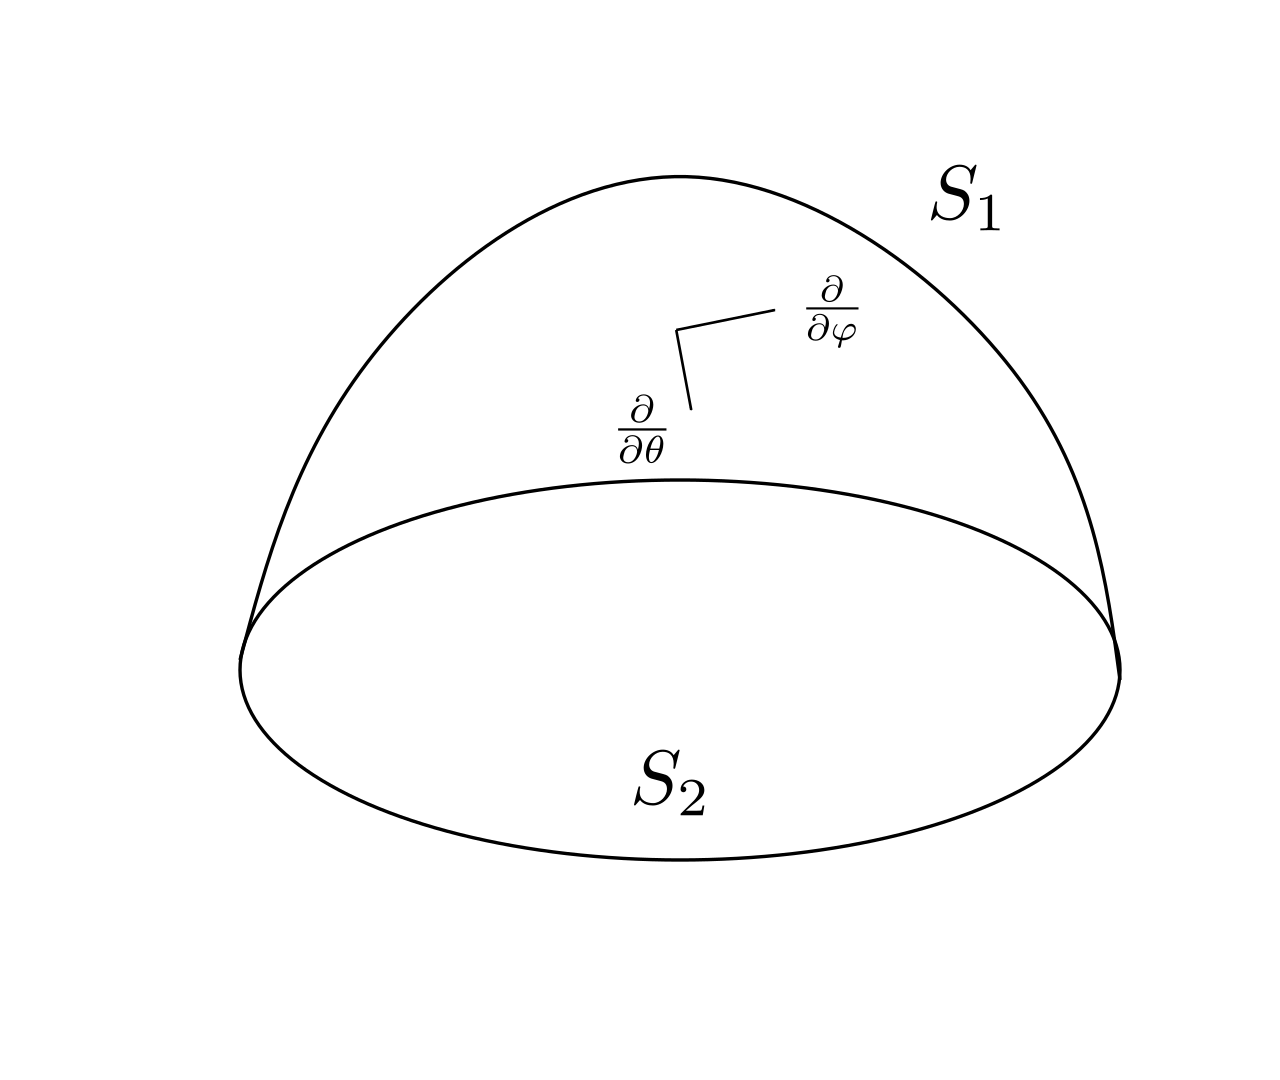
\includegraphics[width=0.4\textwidth]{fig2-6}
        \caption{Tak to wygląda}
        \label{fig:fig2-6}
    \end{figure}
\end{przyklad}
\begin{definicja}
    Atlasem zorientowanym nazywamy taki zbiór otoczeń i map $(U_1, \varphi_1)$, że dla każdej pary $(U_i, \varphi_i), (U_j, \varphi_j)$ takiej, że $U_i\cap U_j \neq \phi$, odwzorowanie $\det\left( \varphi_j \circ \varphi_i^{-1} \right)' > 0$.
\end{definicja}
\begin{definicja}
    Rozmaitość składająca się z atlasu zorientowanego nazywamy orientowalną.
\end{definicja}
\begin{definicja}
    Po wyborze orientacji, rozmaitość nazywamy zorientowaną.
\end{definicja}
\end{document}
